Nachdem nun die konzeptionellen Vorarbeiten geleistet sind, wird in diesem Kapitel die Implementierung des Hyperaudio"=Plugins erläutert. Zu Beginn wird zunächst die grundlegende Struktur des Moodle-Plugins festgehalten. Daraufhin werden das Vorgehen und die Ergebnisse der Implementierung beleuchtet.

%%%%%%%%%%
\section{Struktur des Hyperaudio-Plugins}
\label{sec:architektur}

Die Struktur des Hyperaudio"=Plugins ergibt sich zum einen aus dem durch Moodle vorgegebenen Aufbau eines Plugins, zum anderen durch die gewählte Architektur des Plugins. Beide Bereiche werden in diesem Abschnitt beleuchtet.

\subsubsection{Aufbau eines Moodle-Plugins}
Bei der Implementierung des Hyperaudio"=Plugins ist die durch Moodle vorgegebene Aufbau von Plugins zu beachten \citep{moodle2016activity}. Diese besteht stets aus vorgegebenen Dateien und Ordnern, wobei die jeweilige Anzahl von der Art des zu entwickelnden Plugins abhängig ist. Darüber hinaus bestimmt die Art des Plugins auch den zu wählenden Speicherort.

Bei Activity Plugins, wie dem Plugin für Hyperaudio-Dokumente, ist als Speicherort der Ordner \textbf{/mod} vorgeben. In diesem Ordner muss ein Unterordner mit dem Namen des Plugins angelegt werden, in diesem Fall \textbf{hyperaudio}, in welchem alle Plugin-Dateien abgelegt werden. Eine Übersicht über die Ordnerstruktur des Hyperaudio"=Plugins findet sich in Abbildung \ref{fig:Ordnerstruktur}.

\begin{figure}[h!]
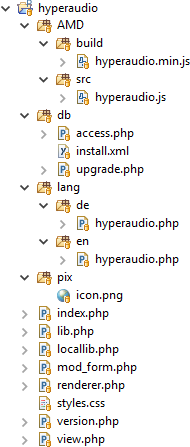
\includegraphics[width=0.3\textwidth,center]{Ordnerstruktur.PNG}
\caption{\label{fig:Ordnerstruktur}Ordnerstruktur des Hyperaudio"=Plugins}
\end{figure}

%\todo[inline]{Ordnerstruktur austauschen}
%\todo[inline]{Warum gibt es hier eine Datei ding.mp3?}

Der Ordner \textbf{/hyperaudio/db} beherbergt die Dateien \textbf{access.php}, \textbf{install.xml} und \textbf{upgrade.php}. Die Datei \textbf{access.php} dient zur Steuerung der Berechtigungen innerhalb des Moodle-Plugins, wobei den verschiedenen Moodle-Rollen verschiedene Rechte für die einzelnen Funktionen zugewiesen werden können. Bei der Installation des Plugins wird die \textbf{install.xml} zur Erstellung der Datenbanktabellen für das Plugin verwendet. Es ist mindestens eine Tabelle mit dem Namen des Plugins anzulegen. Sollten die Datenbanktabellen nach Veröffentlichung des Plugins um Spalten erweitert werden, so kommt die Datei \textbf{upgrade.php} zum Einsatz. Hierin werden die notwendigen Schritte für einen Versionsabgleich definiert.

Im Ordner \textbf{/hyperaudio/lang} wird die Sprachlokalisierung vorgenommen. Für jede Sprache wird innerhalb des \textbf{lang}-Ordners ein eigener Unterordner angelegt. Darin befindet sich jeweils eine PHP-Datei, in welcher die Übersetzungen definiert werden. Der Name dieser Datei entspricht wiederum dem Namen des Plugins.

Das Icon, welches für das Plugin  verwendet werden soll, muss im Ordner \textbf{/hyperaudio/pix} mit dem Dateinamen \textbf{icon.png} abgelegt werden und sollte eine Auflösung von 16x16 Pixel besitzen.

Im Ordner \textbf{/hyperaudio} liegen darüber hinaus die Dateien \textbf{lib.php}, \textbf{mod\underline{{ }}form.php}, \textbf{index.php}, \textbf{view.php} und \textbf{version.php}.\\
Die \textbf{lib.php} dient dazu, Standardfunktionen von Moodle zu überschreiben, wobei \mbox{\texttt{<pluginname>\underline{{ }}add\underline{{ }}instance}}, \texttt{<pluginname>\underline{{ }}update\underline{{ }}instance} und \texttt{<pluginname>\underline{{ }}delete\underline{{ }}instance} als essenzielle Funktionen zu nennen sind. Mit diesen Funktionen wird das Anlegen, Aktualisieren und Löschen von Instanzen des Plugins ermöglicht.\\
Zum Anlegen und Aktualisieren wird in der \textbf{mod\underline{{ }}form.php} die dazugehörige Maske festgelegt.\\
Die \textbf{\textit{index.php}} dient der Auflistung aller Instanzen eines Plugins innerhalb eines Kurses, worüber sich somit eine statistische Ansicht für den jeweiligen Kurs definieren lässt. Je nach Umsetzung kann der Inhalt dieser Auflistung unterschiedlich viele Informationen zu den Instanzen bereitstellen. Auch ist es beispielsweise anhand der Berechtigungen aus der \textbf{access.php} möglich, gewisse Inforationen nur bestimmten Benutzern anzuzeigen.\\
Die erste Datei, die beim Öffnen der Aktivität geladen wird, ist die \textbf{view.php}, welche dementsprechend vornehmlich der Anzeige der Inhalte dient.\\
In der \textbf{version.php} wird die Version des Plugins gepflegt. Erhöht sich die Versionsnummer in der \textbf{version.php}, wird der automatische Upgradeprozess von Moodle für das Plugin ausgelöst.

Neben diesen vorgegebenen Dateien kommen üblicherweise noch weitere Dateien bei der Entwicklung eines Moodle-Plugins zum Einsatz \citep{wild2017moodle}. Dazu gehört beispielsweise die \textbf{locallib.php}, in welcher üblicherweise alle plugineigenen PHP-Funktionen deklariert werden. Auch ist es Usus, die eigentliche Darstellung der Plugin-Inhalte innerhalb eines Kurses von der \textbf{view.php} in eine \textbf{renderer.php} zu verlagern. Dort können verschiedene Renderer-Klassen, welche durch Moodle bereitgestellt werden, für die eigenen Bedürfnisse überschrieben werden. Anpassungen optischer Natur können durch CSS (Cascading Style Sheets) in der \textbf{styles.css} vorgenommen werden. Eigene JavaScript-Module, welche beispielsweise beim Laden der \textbf{view.php} automatisch aufgerufen werden, sind im Verzeichnis \textbf{/hyperaudio/AMD/src} (Asynchronous Module Definition) abzulegen. Für den produktiven Einsatz müssen JavaScript-Module noch minimiert werden. Moodle setzt hierbei auf \textit{Grunt}\footnote{https://gruntjs.com/} \citep{moodle2018grunt}. Die minimierte Version der JavaScript-Module wird im Ordner \textbf{/hyperaudio/AMD/build} abgelegt.

%%%%%%%%%%
\subsubsection{Architektur des Hyperaudio-Plugins}
Basierend auf dem im vorherigen Kapitel beschriebenen Aufbau eines Moodle-Plugins kann nun die Architektur des Hyperaudio"=Plugins dargelegt werden (siehe Abbildung \ref{fig:Architektur}). Das Plugin baut auf der um die für das Hyperaudio"=Plugin benötigten Tabellen erweiterte Datenbank von Moodle auf. Die Renderer (\textbf{view.php}, \textbf{renderer.php}, \textbf{mod\underline{{ }}form.php} und \textbf{index.php}) dienen der Darstellung des User Interfaces und greifen hierfür auf die entsprechenden Daten aus der Datenbank zurück. Während die Renderer die statischen Inhalte des User Interfaces bereitstellen, dient das JavaScript"=Modul (AMD) der Darstellung der dynamischen Inhalte. Hierfür bereitet das JavaScript"=Modul ebenfalls Daten aus der Datenbank auf. Der Zugriff auf die Datenbank erfolgt in diesem Fall aber mittels Webservices. Neben dem Renderer und dem JavaScript-Modul wird das User Interface auch mittels CSS und Thirdparty JavaScript-Frameworks (wie zum Beispiel \textit{Popcorn.js} und \textit{VideoJS}) geformt. Abseits der Darstellung des User Interfaces dienen die Renderer sowie das JavaScript-Modul auch der Verarbeitung von Eingaben im User Interface. Die Core APIs von Moodle unterstützen dabei das Zusammenwirken der verschiedenen Komponenten. Sie ermöglichen beispielsweise die Darstellung von Inhalten sowie direkte Zugriffe auf die Datenbank.

\begin{figure}[h!]
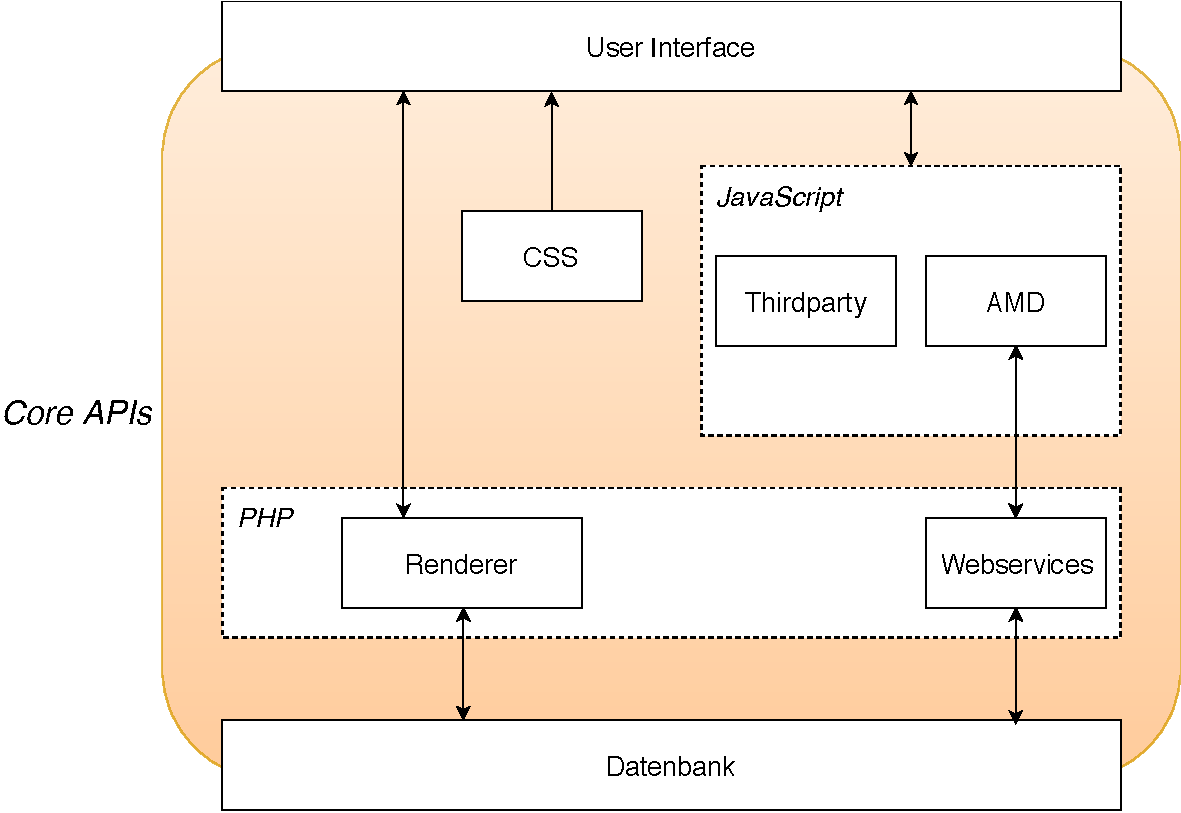
\includegraphics[width=0.70\textwidth,center]{Architektur.PDF}
\caption{\label{fig:Architektur}Architektur des Hyperaudio"=Plugins}
\end{figure} 

%%%%%%%%%%
\section{Iterative Entwicklung}
Die Entwicklung des Plugins wurde in iterativer Form durchgeführt. In jeder Iteration sollte das Plugin nur um einige wenige Funktionalitäten erweitert werden. Jede Iteration sollte mit einem lauffähigen Plugin abgeschlossen werden. So konnte direkt das Ergebnis betrachtet werden und gegebenenfalls in der nächsten Iteration nochmals angepasst werden \citep{augsten2018iterativ}. Die Reihenfolge, in welcher die Funktionalitäten umgesetzt werden, leitete sich aus der Priorisierung der Anforderungen aus Abschnitt \ref{sec:anforderungsdefinition} ab. In den folgenden Abschnitten werden nun die verschiedenen Iterationsschritte vorgestellt. Dabei werden die Kernkonzepte mithilfe von Codeauszügen erläutert.
%\todo[inline]{Ein Hinweis zum Stil: Da es sich bei dieser Textform nicht um ein Manual oder eine technische Dokumentation, sondern eher um einen Bericht der durchgeführten Arbeiten handelt, formuliert man den Text im Präteritum. Angesichts der Tatsache, dass die Iterationen bereits abgeschlossen sind und die Vorgehensweise (Issues, Iterationen, etc.) kaum auf andere Kontexte übertragbar und auch nicht wissenschaftlich relevant sind, muss der Text im Präteritum formuliert sein. }

\subsection{Speichern und Abspielen einer Audio-Datei}
\label{sec:it1}
In der ersten Iteration wurde zunächst die grundlegende Struktur des Plugins erstellt (vgl. Abschnitt \ref{sec:architektur}). Ziel der ersten Iteration sollte es sein, eine Audio-Datei speichern und wiedergeben zu können.

Dazu wurde in der Maske zum Anlegen und Aktualisieren von Instanzen des Hyperaudio"=Plugins (\textbf{mod\underline{{ }}form.php}) neben dem obligatorischen Namens-Feld noch ein Element zum Hinzufügen einer Audio-Datei angelegt. Auflistung \ref{lst:it1:modform} zeigt einen Ausschnitt des Codes, der in der Funktion \texttt{definition} der Klasse \texttt{mod\underline{{ }}hyperaudio\underline{{ }}mod\underline{{ }}form}, die von der Klasse \texttt{moodleform\underline{{ }}mod} erbt, ergänzt werden musste. 

\begin{lstlisting}[language=php,
             linewidth=\textwidth,
             caption={Ausschnitt der \textbf{mod\underline{{ }}form.php} in der 1. Iteration},
             label={lst:it1:modform}]
$mform = $this->_form;
$mform->addElement('text', 'name', get_string('hyperaudio_mod_form_name',
    'hyperaudio'));
$mform->addHelpButton('name', 'hyperaudio_mod_form_name', 'hyperaudio');
$mform->setType('name', PARAM_TEXT);
$mform->addRule('name', get_string('error_wrong_hyperaudio_name_input',
    'hyperaudio'), 'required');
$mform->addElement('filemanager', 'audiofile', get_string('hyperaudiodata',
    'hyperaudio'), null,
    array(
        'subdirs' => 0,
        'maxbytes' => 0,
        'areamaxbytes' => 524288000,
        'maxfiles' => 1,
        'accepted_types' => array(
            'audio'
        )
    ));
$mform->addHelpButton('audiofile', 'hyperaudiodata', 'hyperaudio');
$mform->addRule('audiofile', get_string('required', 'hyperaudio'), 'required');
\end{lstlisting}

Der \texttt{\underline{{ }}form} der \texttt{moodleform\underline{{ }}mod} konnten durch \texttt{addElement} neue Form-Elemente hinzugefügt werden. Mithilfe der Funktionen \texttt{setType}, \texttt{addHelpButton} und \texttt{addRule} konnten den Elementen Datentypen, Hilfe-Button und Regeln zugewiesen werden, die bei Auswertung der Form automatisch validiert werden. Zum Hochladen von Dateien konnte der \textit{filemanager} eingesetzt werden. Mithilfe eines Arrays konnten dabei Einschränkungen für Anzahl und Eigenschaften der hochzuladenden Dateien festgelegt werden. In diesem Fall darf maximal eine Datei hinzugefügt werden, die vom Typ \textit{audio} sein muss. Die Funktion \texttt{get\underline{{ }}string} dient im Allgemeinen der Darstellung der lokalisierten Bezeichnungen.

Um die Daten aus der Form in der Datenbank speichern und später wieder löschen zu können, musste auch die \textbf{lib.php} bearbeitet werden. Dazu dienen die bereits erwähnten Funktionen \texttt{<pluginname>\underline{{ }}add\underline{{ }}instance}, \texttt{<pluginname>\underline{{ }}update\underline{{ }}instance} und \texttt{<pluginname>\underline{{ }}delete\underline{{ }}instance}. Beispielhaft wird in Auflistung \ref{lst:it1:lib} die Funktion \texttt{hyperaudio\underline{{ }}add\underline{{ }}instance} zum Hinzufügen eines neuen Hyperaudio-Dokuments betrachtet. 

\begin{lstlisting}[language=php,
             linewidth=\textwidth,
             caption={Ausschnitt der \textbf{lib.php} in der 1. Iteration},
             label={lst:it1:lib}]
function hyperaudio_add_instance($data) {
    global $DB;
    
    $cmid = $data->coursemodule;
    $context = context_module::instance($cmid);
    
    $draftitemid_audiofile = $data->audiofile;
    unset($data->audiofile);
     
    $now = time();
    $data->timecreated = $now;
    $data->timemodified = $now;
    
    $data->id = $DB->insert_record('hyperaudio', $data);
    
    hyperaudio_update_audiofile($data->id, $context, $draftitemid_audiofile);
     
    return $data->id;
}
\end{lstlisting}

Der Parameter \texttt{\$data} enthält bereits die in der Form eingegebenen Daten. Das Attribut \mbox{\texttt{audiofile}} enthält nicht die Audio-Datei selbst, sondern die ID der \textit{draft file area} und sollte im ersten Schritt nicht in der Tabelle \textit{hyperaudio} abgespeichert werden (vgl. Zeilen 7-8). Vor dem Speichern wird noch der aktuelle Zeitstempel hinterlegt (vgl. Zeilen 10-12). Mithilfe der Funktion \mbox{\texttt{\$DB->insert\underline{{ }}record}} kann das \texttt{\$data}-Objekt mit seinen Attributen in der Tabelle \textit{hyperaudio} abgelegt werden. Im Nachhinein sorgt die in der \textbf{locallib.php} definierte Funktion \mbox{\texttt{hyperaudio\underline{{ }}update\underline{{ }}audiofile}} dafür, dass die Audio-Datei in der \textit{files}-Tabelle abgespeichert und in der \textit{hyperaudio}-Tabelle korrekt referenziert wird (vgl. Auflistung \ref{lst:it1:locallib}).

\begin{lstlisting}[language=php,
             linewidth=\textwidth,
             caption={Ausschnitt der \textbf{locallib.php} in der 1. Iteration},
             label={lst:it1:locallib}]
function hyperaudio_update_audiofile($hyperaudioid, $context, $draftitemid) {
    global $DB;
    
    file_save_draft_area_files($draftitemid, $context->id, 'mod_hyperaudio',
        'audiofile', $hyperaudioid);
    $fs = get_file_storage();
    $files = $fs->get_area_files($context->id, 'mod_hyperaudio', 'audiofile',
        $hyperaudioid, 'itemid, filepath, filename', false);

    $file = reset($files);
    $DB->set_field('hyperaudio', 'audiofile', $file->get_filename(), array(
        'id' => $hyperaudioid
    ));
}
\end{lstlisting}

Wie bereits in Abschnitt \ref{sec:architektur} angedeutet, übernimmt die \textbf{renderer.php} die Anzeige der Hyperaudio-Inhalte (siehe Auflistung \ref{lst:it1:renderer}). Die \textbf{view.php} dagegen reduziert sich auf wenige Zeilen (vgl. Auflistung \ref{lst:it1:view}). Der Plugin-Renderer wird hier benutzt, um Header, Hauptinhalte und Footer anzuzeigen.

\begin{lstlisting}[language=php,
deletekeywords={header},
             linewidth=\textwidth,
             caption={Ausschnitt der \textbf{view.php} in der 1. Iteration},
             label={lst:it1:view}]
$output = $PAGE->get_renderer('mod_hyperaudio');
echo $output->header();
echo $output->display($hyperaudio, $context);
echo $output->footer();
\end{lstlisting}

In der Funktion \texttt{display} der Klasse \mbox{\texttt{mod\underline{{ }}hyperaudio\underline{{ }}renderer}}, die von der Klasse \mbox{\texttt{plugin\underline{{ }}renderer\underline{{ }}base}} erbt, werden die HTML-Inhalte erzeugt. Dabei handelt es sich in der ersten Iteration um einen Container, der ein \texttt{<audio>}-Element beinhaltet. Als Quelle wird im \texttt{<source>}-Element eine URL (Uniform Resource Locator) angegeben, die zuvor mit Moodle-Standardmitteln erzeugt wurde und auf die in der Datenbank abgelegte Audio-Datei verweist.

\begin{lstlisting}[language=php,
             linewidth=\textwidth,
             caption={Ausschnitt der \textbf{renderer.php} in der 1. Iteration},
             label={lst:it1:renderer}]
$audio_fileinfo = array(
    'component' => 'mod_hyperaudio',
    'filearea' => 'audiofile',
    'itemid' => $hyperaudio->id,
    'contextid' => $context->id,
    'filepath' => '/',
    'filename' => $hyperaudio->audiofile
);

$audiofileurl = moodle_url::make_pluginfile_url(
    $audio_fileinfo['contextid'], $audio_fileinfo['component'],
    $audio_fileinfo['filearea'], $audio_fileinfo['itemid'],
    $audio_fileinfo['filepath'], $audio_fileinfo['filename']);
$audio_url = $audiofileurl->get_scheme() . '://' . $audiofileurl->get_host() .
    $audiofileurl->get_path();
if ($audiofileurl->get_port()){
    $audio_url .= ':' . $audiofileurl->get_port();
}
$output = '<div id="hyperaudio"'.
    ' data-hyperaudio_id="'.$hyperaudio->id.'"'.
    ' data-context_id="'.$context->id.'"'.
    ' data-hyperaudio_titel="'.$hyperaudio->name.'"'.
    ' data-hyperaudio_description="'.$hyperaudio->intro.'">';
$output .= '<audio id="hyperaudio_audio" controls>'.
    '<source src="'.$audio_url.'"/>'.
    '</audio>';
$output .= '</div>';

echo $output;
\end{lstlisting}

Auf die beschriebene Art und Weise lies sich ein Hyperaudio-Dokument, das vorläufig allein aus einer Audio-Datei bestand, speichern und mithilfe des HTML5-Audio-Players wiedergeben.


\subsection{Speichern und Anzeige von Zusatzinhalten}
Bei der zweiten Iteration wurde das Plugin um die Möglichkeit zum Speichern und zeitabhängigen Anzeigen der Zusatzinhalte erweitert. Für das Speichern wurde analog zu Abschnitt \ref{sec:it1} vorgegangen. Es wurde ein \textit{filemanager} (\textbf{mod\underline{{ }}form.php}) ergänzt, welcher das Hochladen von beliebig vielen Bilddateien erlaubt. Zusätzlich wurde die \textbf{locallib.php} um die Funktionen \mbox{\texttt{hyperaudio\underline{{ }}update\underline{{ }}additional\underline{{ }}content}} und \mbox{\texttt{hyperaudio\underline{{ }}delete\underline{{ }}additional\underline{{ }}content}} erweitert. Letztere soll verhindern, dass beispielsweise beim Ergänzen von Zusatzinhalten die bereits vorhanden Zusatzinhalte doppelt abgespeichert werden. Dementsprechend wird diese Funktion, wie in Auflistung \ref{lst:it2:locallib} zu sehen, zu Beginn der Funktion \mbox{\texttt{hyperaudio\underline{{ }}update\underline{{ }}additional\underline{{ }}content}} aufgerufen. Die Zeilen 22 bis 27 dienen dazu, die Metadaten des Zusatzinhaltes festzuhalten. In dieser Iteration wurden diese noch mit fixen Beispieldaten befüllt. Die Funktion \mbox{\texttt{hyperaudio\underline{{ }}update\underline{{ }}additional\underline{{ }}content}} wird nun von den Funktionen \texttt{hyperaudio\underline{{ }}add\underline{{ }}instance} und \texttt{hyperaudio\underline{{ }}update\underline{{ }}instance} aufgerufen.

\begin{lstlisting}[language=php,
             linewidth=\textwidth,
             caption={Ausschnitt der \textbf{locallib.php} in der 2. Iteration},
             label={lst:it2:locallib}]
function hyperaudio_update_additional_content
    ($hyperaudioid, $context, $draftitemid, $configfile) {
    global $DB;
    
    hyperaudio_delete_additional_content($hyperaudioid, $context);
    
    file_save_draft_area_files($draftitemid, $context->id,
        'mod_hyperaudio', 'additional_content', $hyperaudioid);
    $fs = get_file_storage();
    
    $files = $fs->get_area_files($context->id, 'mod_hyperaudio',
        'additional_content', $hyperaudioid, 'itemid, filepath, filename',
        false);
    $counter=1;
    $begin=0;
    $end=10;
    foreach ($files as $file) {        
        $additional_content = new \stdClass();
        $additional_content->file = $file->get_filename();
        $additional_content->hyperaudio_id = $hyperaudioid;
        
        $additional_content->name = 'Name '.$counter;
        $additional_content->course_unit = 'Kurseinheit '.$counter;
        $additional_content->page = 'Seite '.$counter;
        $additional_content->description = 'Beschreibung '$counter;
        $additional_content->begin = $begin;
        $additional_content->end = $end;
        
        $now = time();
        $additional_content->timecreated = $now;
        $additional_content->timemodified = $now;
        
        $additional_content_id = $DB->insert_record('additional_content',
            $additional_content);
		
        $counter++;
        $begin+=15;
        $end+=15;
    }
}
\end{lstlisting}

Um die gespeicherten Zusatzinhalte zeitabhängig anzeigen zu können, kommt das JavaScript-Framework \textit{Popcorn.js} zum Einsatz. Dazu wurden die JavaScript-Dateien von \textit{Popcorn.js} und dessen \textit{Images}-Plugin im Ordner \textbf{/hyperaudio/thirdparty} abgelegt und in die \textbf{view.php} eingebunden (siehe Auflistung \ref{lst:it2:view}).

\begin{lstlisting}[language=php,
             linewidth=\textwidth,
             caption={Ausschnitt der \textbf{view.php} in der 2. Iteration},
             label={lst:it2:view}]
$PAGE->requires->js('/mod/hyperaudio/thirdparty/popcorn.js', true);
$PAGE->requires->js('/mod/hyperaudio/thirdparty/popcorn.image.js', true);
\end{lstlisting}

Im Renderer wurde ein weiteres \texttt{<div>}-Element ergänzt, in welchem die Zusatzinhalte angezeigt werden sollen. Diese werden aus der Datenbank geladen und in einer Schleife abgearbeitet. Dabei wird zunächst eine URL zur Bilddatei generiert. Über \texttt{popcorn.image} sorgt das \textit{Popcorn.js} \textit{Images}-Plugin dafür, dass diese URL zu den definierten Zeitpunkten abgerufen und das entsprechende Bild angezeigt wird (vgl. Zeilen 50-55).

\begin{lstlisting}[language=php,
             linewidth=\textwidth,
             caption={Ausschnitt der \textbf{renderer.php} in der 2. Iteration},
             label={lst:it2:renderer}]
$output = '<div id="hyperaudio"'.
    ' data-hyperaudio_id="'.$hyperaudio->id.'"'.
    ' data-context_id="'.$context->id.'"'.
    ' data-hyperaudio_titel="'.$hyperaudio->name.'"'.
    ' data-hyperaudio_description="'.$hyperaudio->intro.'">';
$output .= '<div id="hyperaudio_additional_content"></div>';
$output .= '<audio id="hyperaudio_audio" controls>' .
    '<source src="'.$audio_url.'"/>'.
    '</audio>';

$output .= '<script type="text/javascript">'.
    'document.addEventListener("DOMContentLoaded", function() {'.
        'var popcorn = Popcorn("#hyperaudio_audio");';

$files = hyperaudio_get_additional_content($hyperaudio->id, $context);
foreach ($files as $file) {
    $additional_content = $DB->get_record('additional_content',
        array(
            'hyperaudio_id' => $hyperaudio->id,
            'file' => $file->get_filename()
	    ),'*', IGNORE_MISSING);
        
    if ($additional_content == false){
        continue;
	}
	
    $additional_content_fileinfo = array(
        'component' => 'mod_hyperaudio',
        'filearea' => 'additional_content',
        'itemid' => $hyperaudio->id,
        'contextid' => $context->id,
        'filepath' => '/',
        'filename' => $additional_content->file
    );
	
    $additional_content_fileurl = moodle_url::make_pluginfile_url(
        $additional_content_fileinfo['contextid'],
        $additional_content_fileinfo['component'],
        $additional_content_fileinfo['filearea'],
        $additional_content_fileinfo['itemid'],
        $additional_content_fileinfo['filepath'],
        $additional_content_fileinfo['filename']);
        $additional_content_url = $additional_content_fileurl->get_scheme() .'://'.
        $additional_content_fileurl->get_host() . 
        $additional_content_fileurl->get_path();
    if ($additional_content_fileurl->get_port()){
        $additional_content_url .= ':'. $additional_content_fileurl->get_port();
    }
	
    $output .= 'popcorn.image({'.
        ' start: '.$additional_content->begin.','.
        ' end: '.$additional_content->end.','.
        ' href: "javascript:void(0);",'.
        ' src: "'.$additional_content_url.'",'.
        ' target: "hyperaudio_additional_content"});';
}

$output .= '}, false);</script>';
$output .= '</div>';

echo $output;
\end{lstlisting}

Mit diesen Erweiterungen wurde das Ziel der zweiten Iteration erreicht. Es war nun möglich, Zusatzinhalte abzuspeichern und diese unter Verwendung von \textit{Popcorn.js} zeitabhängig zur Audio-Datei darstellen zu lassen.

\subsection{Einbindung der Konfigurationsdatei}
Damit die Beispieldaten durch tatsächliche Metadateninformationen ausgetauscht werden konnte, war in der dritten Iteration die Einbindung der Konfigurationsdatei notwendig. Zu Beginn dieser Iteration stand erneut die Erweiterung der \textbf{mod\underline{{ }}form.php} um einen weiteren \textit{filemanager}, der maximal eine Konfigurationsdatei im JSON-Format entgegennimmt. Die Speicherung verläuft analog zur Speicherung der Zusatzinhalte. In diesem Zuge wurden also erneut die \textbf{lib.php} und \textbf{locallib.php} entsprechend erweitert. Neben den Funktionen \texttt{hyperaudio\underline{{ }}update\underline{{ }}hyperaudio\underline{{ }}config} und \texttt{hyperaudio\underline{{ }}delete\underline{{ }}hyperaudio\underline{{ }}config} wurde, wie in Auflistung \ref{lst:it3:locallib} zu erkennen, die Funktion \texttt{hyperaudio\underline{{ }}update\underline{{ }}additional\underline{{ }}content} erweitert. Es ist zu entnehmen, dass zunächst die Inhalte der Konfigurationsdatei mithilfe der Funktion \texttt{hyperaudio\underline{{ }}parse\underline{{ }}hyperaudio\underline{{ }}config} ausgelesen werden, um diese Metadaten dann beim Abspeichern der Zusatzinhalte zu verwenden.

\begin{lstlisting}[language=php,
             linewidth=\textwidth,
             caption={Ausschnitt der \textbf{locallib.php} in der 3. Iteration},
             label={lst:it3:locallib}]
hyperaudio_update_additional_content($hyperaudio_id, $context,
    $draftitemid, $configfile){
	
    //...
	
    $additional_contents_data = 
        hyperaudio_parse_hyperaudio_config($hyperaudioid, $context, $configfile)
                ["additional_contents_by_filename"];
    
    //...
	
    foreach ($files as $file) {        
        //...
        
        $additional_content_data =
            $additional_contents_data[$additional_content->file];
        
        $additional_content->name = $additional_content_data->name;
        $additional_content->course_unit = $additional_content_data->course_unit;
        $additional_content->page = $additional_content_data->page;
        $additional_content->description = $additional_content_data->description;
        $additional_content->begin = $additional_content_data->begin;
        $additional_content->end = $additional_content_data->end;
        
        //...
    }    
}

//...

function hyperaudio_parse_hyperaudio_config($hyperaudio_id, $context, $configfile) {
    
    $fs = get_file_storage();
    $file = $fs->get_file(
        $context->id, 'mod_hyperaudio', 'hyperaudio_config',
        $hyperaudio_id, '/', $configfile);
    $jsontext = $file->get_content();
    $json = json_decode ($jsontext);
    
    $hyperaudio_author = $json->author;
    
    $additional_contents = $json->additional_contents->additional_content;
    $additional_contents_by_filename =
        array_column($additional_contents, NULL, 'filename');
    
    return array(
        'additional_contents_by_filename' => $additional_contents_by_filename,
        'hyperaudio_author' => $hyperaudio_author);
}
\end{lstlisting}



Als Ergebnis dieser Iteration konnten nun Zusatzinhalte zu den Zeitpunkten dargestellt werden, welche in der Konfigurationsdatei definiert sind.

\subsection{Speichern und Anzeige von Kommentaren}
\label{sub:SpeichernKommentare}
Nachdem in den vorherigen Iterationen die Pflege und das Abspielen von Hyperaudio-Dokumenten im Fokus lag, konzentrierte sich diese Iteration auf die Kommentarfunktion. Zu diesem Zweck wurde im ersten Schritt der Renderer um entsprechende Elemente ergänzt, welche in Auflistung \ref{lst:it4:renderer} zu sehen sind. Dabei handelt es sich zum einen um eine Textarea mit dazugehörigem Submit-Button, welche dem Erstellen von Kommentaren dienen. Das \texttt{<div>}-Element mit der ID \mbox{\textit{hyperaudio\underline{{ }}comments}} soll der Anzeige der Kommentare dienen.

\begin{lstlisting}[language=php,
             linewidth=\textwidth,
             caption={Ausschnitt der \textbf{renderer.php} in der 4. Iteration},
             label={lst:it4:renderer}]
$output .=
    '<div id="comment_creation_container" class="textarea_container">'.
        '<textarea id="hyperaudio_comment" name="hyperaudio_comment"'.
            ' class="hyperaudio_textarea" autocomplete="off"'.
            ' placeholder="'.
                get_string('mod_hyperaudio_renderer_comment', 'hyperaudio').
            '...'.'">'.
        '</textarea>'.
        '<button type="button" class="comment_submit"'.
            ' data-comment_type="'.CommentType::Comment.'">'.
                get_string('mod_hyperaudio_renderer_submit_comment', 'hyperaudio').
        '</button>'.
    '</div>';
$output .= '<div id="hyperaudio_comments"></div>';
\end{lstlisting}

Das Speichern sowie das Anzeigen der Kommentare wurde unter Einsatz von Webservices, welche durch ein JavaScript-Modul (\textbf{/hyperaudio/AMD/src/hyperaudio.js}) angesprochen werden, realisiert. Hierfür wurden zusätzlich die Dateien \textbf{services.php} (\textbf{/hyperaudio/db}) und \textbf{external.php} (\textbf{/hyperaudio/classes}) für die Bereitstellung der Webservices benötigt.

In der \textbf{services.php} wurden zunächst die nötigen Webservices deklariert (siehe Auflistung \ref{lst:it4:services}). Hier wird lediglich auf die \textbf{external.php} verwiesen, die den eigentlichen Code der Webservices beinhalten.

\begin{lstlisting}[language=php,
             linewidth=\textwidth,
             caption={Ausschnitt der \textbf{services.php} in der 4. Iteration},
             label={lst:it4:services}]
$functions = array(
    'mod_hyperaudio_save_comment' => array(
        'classname'   => 'mod_hyperaudio_external',
        'methodname'  => 'save_comment',
        'classpath'   => 'mod/hyperaudio/classes/external.php',
        'description' => 'Save comment',
        'type'        => 'write'
    ),
    'mod_hyperaudio_load_comments' => array(
        'classname'   => 'mod_hyperaudio_external',
        'methodname'  => 'load_comments',
        'classpath'   => 'mod/hyperaudio/classes/external.php',
        'description' => 'Load comments',
        'type'        => 'read'
    )
);
\end{lstlisting}

In der \textbf{external.php} wurden in der Funktion \texttt{mod\underline{{ }}hyperaudio\underline{{ }}external}, welche von der Klasse \texttt{external\underline{{ }}api} erbt, die Webservice-Funktionen definiert. Dabei sind für einen Webservice jeweils vier Funktionen von Nöten:

\begin{itemize}
\item \texttt{<webservice\underline{{ }}name>\underline{{ }}parameters}: definiert die Eingabe-Parameter des Webservices
\item \texttt{<webservice\underline{{ }}name>\underline{{ }}is\underline{{ }}allowed\underline{{ }}from\underline{{ }}ajax}: definiert, ob der Webservice über AJAX (Asynchronous JavaScript and XML) aufgerufen werden kann
\item \texttt{<webservice\underline{{ }}name>}: Hauptfunktion, welche die Eingabe-Parameter verarbeitet und ein Ergebnis zurückliefert
\item \texttt{<webservice\underline{{ }}name>\underline{{ }}returns}: definiert die Struktur der Rückgabewerte des Webservices
\end{itemize}

Auflistung \ref{lst:it4:external} zeigt exemplarisch die Umsetzung des Webservices \texttt{load\underline{{ }}comments}. Anhand der übergebenen \texttt{\$hyperaudio\underline{{ }}id} werden die Kommentare mittels SQL (Structured Query Language) aus der Datenbank gelesen und in einer aufbereiteten Struktur zurückgegeben.

\begin{lstlisting}[language=php,
             linewidth=\textwidth,
             caption={Ausschnitt der \textbf{external.php} in der 4. Iteration},
             label={lst:it4:external}]
class mod_hyperaudio_external extends external_api {
    
    public static function load_comments_parameters() {
        return new external_function_parameters(
            array(
            'hyperaudio_id' => new external_value(PARAM_INT, 'hyperaudio_id')
            )
        );
    }
    
    public static function load_comments_is_allowed_from_ajax() {
        return true;
    }
    
    public static function load_comments($hyperaudio_id) {
        global $CFG, $DB;
        
        require_once ($CFG->dirroot . '/mod/hyperaudio/locallib.php');
        require_once ($CFG->dirroot . '/mod/hyperaudio/classes/enums.php');
        
        $comments = $DB->get_records_sql(
            'SELECT comments.id, comments.comment_type,'.
            ' comments.commenttext, comments.timeannotated,'.
            ' comments.timecreated, user.username'.
            ' FROM mdl_hyperaudio_comments comments'.
            ' INNER JOIN mdl_user user ON comments.userid = user.id'.
            ' WHERE comments.hyperaudio_id = ?'.
            ' AND (comments.comment_type = ? )'.
            ' ORDER BY comments.timecreated',
            array($hyperaudio_id, CommentType::Comment)
        );
        
        $result_comments = array();
        foreach ($comments as $comment) {
            $result_comment = array(
                'id' => $comment->id,
                'username' => $comment->username,
                'date' => date('d.m.Y H:i', $comment->timecreated),
                'time' => format_time_annotated($comment->timeannotated),
                'text' => $comment->commenttext,
                'comment_type' => $comment->comment_type
            );
            $result_comments[] = $result_comment;
        }
        
        return $result_comments;
    }
    
    public static function load_comments_returns() {
        return new external_multiple_structure(
            new external_single_structure(
                array(
                    'id' => new external_value(PARAM_INT, 'id'),
                    'username' => new external_value(PARAM_TEXT, 'username'),
                    'date' => new external_value(PARAM_TEXT, 'date'),
                    'time' => new external_value(PARAM_TEXT, 'time'),
                    'text' => new external_value(PARAM_TEXT, 'text'),
                    'comment_type' => new external_value(PARAM_TEXT, 'comment_type')
                )
            )
        );
    }
}             
\end{lstlisting}

Für den Zugriff auf die Webservices wurde das JavaScript-Modul \textbf{hyperaudio.js}, welches sich im Ordner \textbf{/hyperaudio/AMD} befindet, eingeführt. Das Modul dient dazu die im Renderer definierten Elemente zu befüllen beziehungsweise auszulesen.
Die Funktion zum Speichern eines Kommentars ist exemplarisch in Auflistung \ref{lst:it4:hyperaudio} dargestellt. Zunächst werden die im Renderer erstellten Elemente zum Erstellen eines Kommentars ausgelesen. Um Funktionen die mehrfach benötigt werden, wie die Funktion \texttt{get\underline{{ }}hyperaudio\underline{{ }}id},  auszugliedern, wurde die Datei \textbf{locallib.js} im Ordner \textbf{/hyperaudio/thirdparty} implementiert. Nachdem die Elemente ausgelesen wurden, wird mittels eines AJAX-Calls der Webservice \texttt{mod\underline{{ }}hyperaudio\underline{{ }}save\underline{{ }}comment} aufgerufen und die benötigten Parameter übergeben. Hierbei ist hervorzuheben, dass der Zeitpunkt, zu dem der Kommentar an das Hyperaudio-Dokument annotiert wird, über die Funktion \texttt{currentTime} des \textit{Popcorn.js}-Frameworks ermittelt werden kann. Bei der Funktion \texttt{show\underline{{ }}comments} zum Darstellen der Kommentare wurde analog vorgegangen, nur dass durch den Webservice die Kommentare für das betroffene Hyperaudio-Dokumente abgefragt und innerhalb des dazugehörigen Elements des Renderers dargestellt werden.


\begin{lstlisting}[language=php,
             linewidth=\textwidth,
             caption={Ausschnitt der \textbf{hyperaudio.js} in der 4. Iteration},
             label={lst:it4:hyperaudio}]
function save_comment(comment_type){
    var comment = $("#hyperaudio_comment").val();
    var hyperaudio_id = get_hyperaudio_id();
    var popcorn = Popcorn("#hyperaudio_audio");
    var timeannotated = popcorn.currentTime();
    timeannotated = parseInt(timeannotated);
	    
    var promises = ajax.call([{
        methodname: 'mod_hyperaudio_save_comment',
        args:{
            'comment': comment,
            'hyperaudio_id': hyperaudio_id,       
            'timeannotated': timeannotated,
            'comment_type': comment_type
        }
    }]);
    promises[0].done(function(data) {
        show_comments();
    });
}
\end{lstlisting}

\begin{lstlisting}[language=php,
             linewidth=\textwidth,
             caption={Ausschnitt der \textbf{locallib.js} in der 4. Iteration},
             label={lst:it4:locallib.js}]
function get_hyperaudio_id(){
    return $("#hyperaudio").attr("data-hyperaudio_id");
}
function jump_to_time(element){
    var time = $(element).attr("data-annotated_time");
    var popcorn = get_popcorn();
    popcorn.currentTime(time);
    popcorn.play();
}
\end{lstlisting}

In der \textbf{locallib.js} ist darüber hinaus mit \texttt{jump\underline{{ }}to\underline{{ }}time} eine Funktion enthalten, mit welcher die Rückkopplung an die Mediensteuerung ermöglicht wurde.

Mit dem Abschluss dieser Iteration wurde die Möglichkeit geschaffen, Kommentare zu verfassen und dabei den Zeitpunkt innerhalb des Hyperaudio-Dokuments festzuhalten, zu dem der Kommentar erstellt wurde. Im gleichen Zuge wurde auch die Darstellung dieser Kommentare ermöglicht.

\subsection{Antworten auf Kommentare}
Im nächsten Schritt sollte nun eine Antwortmöglichkeit auf Kommentare geschaffen werden. Zu diesem Zweck wurde ein neuer Webservices zum Speichern von Antworten erstellt und der Webservice zum Darstellen der Kommentare um Antworten erweitert. Bei der \textbf{hyperaudio.js} bedurfte es ebenfalls nur kleinerer Anpassungen, um unter anderem die Anzeige eines Antworten-Buttons und eines Textfeldes bei dessen Betätigung zu ermöglichen (siehe Abbildung \ref{fig:Antworten}). Die hierfür notwendige Erweiterung innerhalb der Funktion \texttt{show\underline{{ }}comments} ist in der Auflistung \ref{lst:it5:hyperaudio} zu sehen.

\begin{figure}[h!]
\begin{subfigure}[c]{0.5\textwidth}
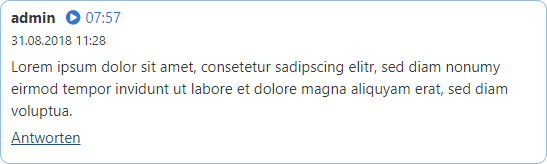
\includegraphics[width=0.95\textwidth,center]{Antworten1.png}
\label{fig:Antworten1}
\end{subfigure}%
\begin{subfigure}[c]{0.5\textwidth}
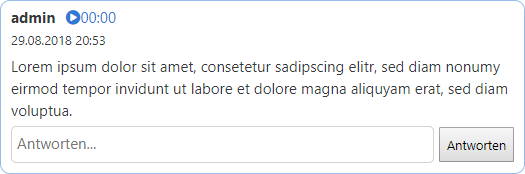
\includegraphics[width=0.95\textwidth,center]{Antworten2.png}
\label{fig:Antworten2}
\end{subfigure}
\caption{Darstellung der Antworten-Funktion}
\label{fig:Antworten}
\end{figure}

\begin{lstlisting}[language=php,
             linewidth=\textwidth,
             caption={Ausschnitt der \textbf{hyperaudio.js} in der 5. Iteration},
             label={lst:it5:hyperaudio}]
if (this.comment_type === CommentType.Comment && !this.comment_id){
    output = output + '<div' +
        ' class="comment_answer comment_actions"' +
        ' data-comment_id="' + this.id + '">';
    output = output + '<a href="javascript:void(0);"' +
        ' class="comment_answer_link comment_link active"' +
        ' onclick="show_answer_textarea(this)"' +
        ' data-comment_id="' + this.id + '">' + string_answer + '</a>';
    output = output + '<div class="textarea_container">';
    output = output + '<textarea' +
        ' class="comment_answer_text comment_hidden_element hyperaudio_textarea"' +
        ' data-comment_id="' + this.id + '" ' + 
        ' placeholder="' + string_answer + '...' + '"/>';
    output = output + '<button type="button"' +
        ' class="comment_answer_button comment_hidden_element' +
        ' hyperaudio_comment_button"' +
       '  data-comment_id="' + this.id + '">' + string_answer + '</button>';
    output = output + '</div>';
    output = output + '</div>';
\end{lstlisting}

Durch die Erweiterungen und Anpassungen innerhalb dieser Iteration war es nun möglich auf Kommentare zu antworten und diese Antwort beim zugehörigen Kommentar darzustellen.

\subsection{Notizen}
\label{sub:notizen}
Nachdem durch die vorangegangenen Iterationen nun die Funktionen für die Kommunikation zwischen Studierenden und Lehrenden geschaffen wurden, zielte diese Iteration auf das Erstellen und Darstellen von Notizen ab.

Zum Speichern der Notizen konnten dieselben Webservices und Funktionen, wie zum Speichern der Kommentare verwendet werden. Dies rührt daher, dass Notizen eine bestimmte Art von Kommentaren darstellen (vgl. Abschnitt \ref{sec:komponenten_zusammenhaenge}). 

Da Notizen im Gegensatz zu Kommentaren geändert und gelöscht werden können sollen, mussten hierfür entsprechende Webservices bereitgestellt werden. Gleichzeitig mussten analog zum Antworten auf Kommentare ein Button zum Löschen sowie Button und Textfeld für die Bearbeitung der Notiz ergänzt werden (siehe Auflistung \ref{lst:it6:hyperaudio}). 

Die Darstellung des Schloss-Symbols als Symbol für Notizen wurde mithilfe der schriftbasierten Icon-Sammlung \textit{Font Awesome}\footnote{https://fontawesome.com/} realisiert.

\begin{figure}[h!]
\begin{subfigure}[c]{0.5\textwidth}
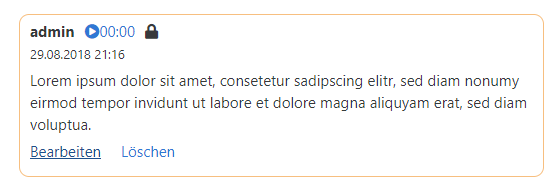
\includegraphics[width=0.95\textwidth,center]{Notiz1.png}
\label{fig:Notiz1}
\end{subfigure}%
\begin{subfigure}[c]{0.5\textwidth}
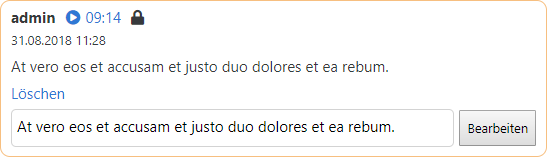
\includegraphics[width=0.95\textwidth,center]{Notiz2.png}
\label{fig:Notiz2}
\end{subfigure}
\caption{Darstellung der Notiz-Funktion}
\label{fig:Notiz}
\end{figure}

\begin{lstlisting}[language=php,
             linewidth=\textwidth,
             caption={Ausschnitt der \textbf{hyperaudio.js} in der 6. Iteration},
             label={lst:it6:hyperaudio}]
else if (this.comment_type === CommentType.Note){
    output = output + '<div' +
        ' class="comment_note comment_actions" data-comment_id="' + this.id + '">';
    output = output + '<a href="javascript:void(0);"' +
        ' class="comment_note_edit_link comment_link active"' +
        ' onclick="show_note_edit_textarea(this)"' +
        ' data-comment_id="' + this.id + '">' + string_edit + '</a>';
    output = output + '<a href="javascript:void(0);"' +
        ' class="comment_note_delete_link comment_link active"' +
        ' data-comment_id="' + this.id + '">' + string_delete + '</a>';
    output = output + '<div class="textarea_container">';
    output = output + '<textarea' +
        ' class="comment_note_edit_text comment_hidden_element' +
        ' hyperaudio_textarea"' +
        ' data-comment_id="' + this.id + '">' + this.text + '</textarea>';
    output = output + '<button type="button"' +
        ' class="comment_note_edit_button comment_hidden_element' +
        ' hyperaudio_comment_button"' +
        ' data-comment_id="' + this.id + '">' + string_edit + '</button>';
    output = output + '</div>';
    output = output + '</div>';
}		
\end{lstlisting}

Entsprechend der Webservices wurden innerhalb der \textbf{external.php} Funktionen zum Editieren von Notizen und dem Löschen von Kommentaren erstellt. Damit waren alle nötigen Schritte durchgeführt um Notizen erstellen, anzeigen und löschen zu können.


\subsection{Audio Cues}
Das Abspielen der Audio Cues im Moment der Darstellung eines Zusatzinhaltes wurde durch eine Erweiterung des verwendeten \textit{Popcorn.js}-Plugin \textit{Images} erreicht. In diesem Zug wurde das \textit{Popcorn.js}-Plugin \textit{Hyperaudio} basierend auf dem \textit{Images}-Plugin entwickelt.

Hierfür wurde in den Optionen ein zusätzlicher Parameter \texttt{cue} eingeführt. Dieser nimmt die ID eines \texttt{<audio>}-Elements entgegen, welches den abzuspielenden Audio Cue wiedergeben kann (vgl. Auflistung \ref{lst:it7:renderer}). Um den Ton zeitgleich mit der Anzeige des Zusatzinhaltes abzuspielen, wurde eine Anpassung in der Funktion \texttt{start} vorgenommen. Sofern keine Stummschaltung oder Pausierung des Hyperaudio-Dokuments vorliegt, wird die Wiedergabe des Audio Cues durch den Aufruf der \texttt{play}-Funktion des HTML5-Audioplayers angestoßen. Auflistung \ref{lst:it7:popcorn.hyperaudio} zeigt die Erweiterungen des \textit{Popcorn.js}-Plugins \textit{Hyperaudio}.
%\todo[inline]{Wenn ich das richtig verstehe, gibt es ein einziges Tonsignal für alle Arten von Annotationen. Wie soll der Nutzer erkennen, ob an der gegenwärtigen Abspielposition ein Komentar, eine Notitz oder ein Medienelement hinterlegt ist?}

\begin{lstlisting}[language=php,
             linewidth=\textwidth,
             caption={Ausschnitt der \textbf{renderer.php} in der 7. Iteration},
             label={lst:it7:renderer}]
$output .= '<audio id="hyperaudio_audio_cue"'.
    ' src="../hyperaudio/audiocues/ding.mp3"></audio>';

//...

$output .= 'popcorn.hyperaudio({'.
        ' start: '.$additional_content->begin.','.
        ' end: '.$additional_content->end.','.
        ' href: "javascript:void(0);",'.
        ' src: "'.$additional_content_url.'",'.
        ' target: "hyperaudio_additional_content",'.
        ' cue: "hyperaudio_audio_cue"});';
\end{lstlisting}

\begin{lstlisting}[language=php,
             linewidth=\textwidth,
             caption={Ausschnitt der \textbf{popcorn.hyperaudio.js} in der 7. Iteration},
             label={lst:it7:popcorn.hyperaudio}]
options: {

    //...
    
    cue: "audio-cue",

    //...    
    
}

//...

start: function( event, options ) {
    options.anchor.style.display = "inline";
    if ( options.trackedContainer ) {
        options.trackedContainer.start();
    }
    var audioElement = document.getElementById( options.cue );
    if (!this.media.muted && !this.media.paused){
        audioElement.play();
    }
},
\end{lstlisting}

Durch die Weiterentwicklung des \textit{Images}-Plugins zum \textit{Popcorn.js}-Plugin \textit{Hyperaudio} wurde in dieser Iteration die Wiedergabe von Audio Cues beim Anzeigen von Zusatzinhalten implementiert.

\subsection{Galerie der Zusatzinhalte}
Der Anforderung nach einer Übersicht über annotierte Zusatzinhalte wurde mittels einer Galerie begegnet, welche in dieser Iteration umgesetzt wurde. Hierfür wurden in der \textbf{renderer.php} zunächst die Metainformationen zu allen Zusatzinhalten des Hyperaudio-Dokuments geladen, um anhand dieser im nächsten Schritt URLs zu den Zusatzinhalten zu generieren. Damit wurde eine Darstellung gemäß der Idee aus Abbildung \ref{fig:MockupGalerieFinal} umgesetzt (siehe Abbildung \ref{fig:Galerie}). Die Rückkopplung zur Mediensteuerung erfolgte wie bereits bei den Kommentaren mithilfe der \texttt{jump_to_time}-Funktion.

\begin{figure}[h!]
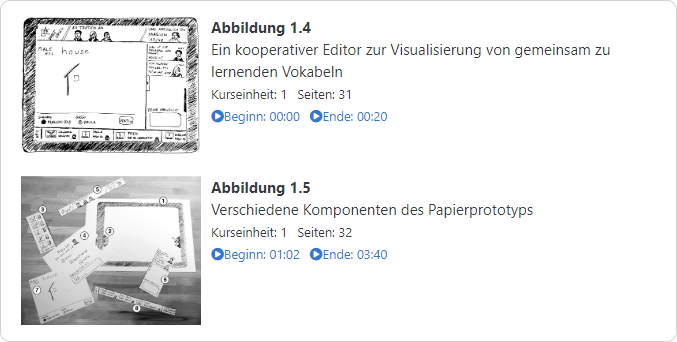
\includegraphics[width=0.8\textwidth,center]{Galerie.png}
\caption{\label{fig:Galerie}Darstellung der Galerie}
\end{figure}


Um eine vergrößerte Darstellung der Zusatzinhalte zu realisieren, wurde ein versteckter Bereich angelegt. Beim Klick auf ein Vorschaubild wird mithilfe der Funktion \texttt{show\underline{{ }}modal} der entsprechende Zusatzinhalt in diesen Bereich geladen und dargestellt (vgl. Auflistung \ref{lst:it8:hyperaudio}). 

\begin{lstlisting}[language=php,
             linewidth=\textwidth,
             caption={Ausschnitt der \textbf{hyperaudio.js} in der 8. Iteration},
             label={lst:it8:hyperaudio}]
function show_modal(source, caption){
    $("#hyperaudio_modal_image").attr("src", source);
    $("#hyperaudio_modal_caption").html(caption);
    $("#hyperaudio_modal").css("display", "block");
}
\end{lstlisting}

Durch diese Implementierung wurde die Darstellung der Galerie erreicht, durch Verwendung der JavaScript-Funktion \texttt{jump\underline{{ }}to\underline{{ }}time} wurde zusätzlich noch die Rückkopplung an die Mediensteuerung geboten. 

\subsection{Zeitabhängige Visualisierung der Kommentare und Notizen}
In dieser Iteration sollte sich nun der zeitabhängigen Visualisierung der Kommentare und Notizen zugewendet werden. An dieser Stelle muss festgehalten werden, dass dies beim Einsatz des Standard HTML5-Audioplayers schwer umsetzbar gewesen wäre, weshalb auf die Erkenntnisse bezüglich des \textit{VideoJS Players} aus Abschnitt \ref{sub:TechnologienMoodle} zurückgegriffen wurde. Die umfassenden Anpassungsmöglichkeiten sollten sich nun in dieser Iteration zu Nutze gemacht werden.

Im ersten Schritt wurden zunächst die benötigten Informationen für die Darstellung der in Abbildung \ref{fig:MockupMediensteuerungV3} beschriebenen Blöcke aus der Datenbank abgerufen. Hierfür wurde ein neuer Webservice eingeführt und unter anderem  die \textbf{external.php} erweitert.

Um die ermittelten Informationen darzustellen, wird, wie in Auflistung \ref{lst:it9:hyperaudio} zu erkennen, der Webservice von der Funktion \texttt{show\underline{{ }}timeline} der \textbf{hyperaudio.js} aufgerufen und darauf die Größe der Blöcke unter Berücksichtigung der Größe der Timeline berechnet. Dabei wird auf vorhandene HTML Elemente des \textit{VideoJS Players} zurückgegriffen, um die gewünschte Darstellung der Blöcke ober- und unterhalb der Timeline zu erreichen.

\begin{lstlisting}[language=php,
             linewidth=\textwidth,
             caption={Ausschnitt der \textbf{hyperaudio.js} in der 9. Iteration},
             label={lst:it9:hyperaudio}]
var promises = ajax.call([{
    methodname: 'mod_hyperaudio_load_timeline_comments',
    args:{
        'hyperaudio_id': hyperaudio_id,
        'duration': duration,
        'number_of_slots': number_of_slots
        }
    }]);
promises[0].done(function(data) {
    var container_height =
        $(".hyperaudio_timeline_blocks_container.comment_blocks_container").
            height();
		    	
    var pixel_width = 
        ((container_width - (number_of_slots - 1) * 2 * 2) / number_of_slots);
    var width = (pixel_width / (container_width + 20)) * 100;
    var height_1_comment = ((container_height - 5) / data.max_count);
		    	
    var output_comments = '';
    var output_notes = '';
    var height;
    var class_zero;
		    	
    function set_height_and_class(annotations){
        height = annotations * height_1_comment;
        if (height == 0){
            class_zero = 'block_zero';
        }
        else {
            class_zero = '';
        }
        if (height < 5){
            height = 5;
        }
    }
		    	
    function get_title(title, username){
        var result_title = '';
		    		
        if (username){
            result_title = username + ':\n';
        }
		    		
        if (title){
            if (title.length > 100){
                result_title = result_title + title.substr(0, 100) + " ...";
            }
            else {
                result_title = result_title + title;
            }
        }
		    		
        return result_title;
    }
		    	
    $(data.blocks).each(function(){
        set_height_and_class(this.comments);
        output_comments = output_comments + 
            '<div title="' + 
            get_title(this.title_comment_text, this.title_comment_username) + '"' +
            ' class="timeline_block comment_block ' + class_zero + '"' +
            ' data-comment-id="' + this.title_comment_id + '"' +
            ' style="width: ' + width + '%; height: ' + height + 'px;"' +
            ' onclick="jump_to_comment(this)"></div>';
                
        set_height_and_class(this.notes);
        output_notes = output_notes +
            '<div title="' + get_title(this.title_note_text) + '"' +
            ' class="timeline_block note_block ' + class_zero + '"' +
            ' data-comment-id="' + this.title_note_id + '"' +
            ' style="width: ' + width + '%; height: ' +	height + 'px;"' +
            ' onclick="jump_to_comment(this)"></div>';
    });
    $(".hyperaudio_timeline_blocks.comment_blocks").html(output_comments);
    $(".hyperaudio_timeline_blocks.note_blocks").html(output_notes);
});
\end{lstlisting}
Beim Klick auf einen Block wird mit der Funktion \texttt{jump\underline{{ }}to\underline{{ }}comment} zu dem Kommentar gesprungen, welcher im Tooltip dargestellt wird. Selbiges gilt für Notizen. Hierbei mussten, wie in Auflistung \ref{lst:it9:locallib.js} zu sehen, auch Standard-Moodle-Elemente (Titelleiste) berücksichtigt werden, um die korrekte Stelle zu ermitteln, zu der gesprungen werden muss.

\begin{lstlisting}[language=php,
             linewidth=\textwidth,
             caption={Ausschnitt der \textbf{locallib.js} in der 9. Iteration},
             label={lst:it9:locallib.js}]
function jump_to_comment(element){
    var comment_id = $(element).attr("data-comment-id");
	
    if (comment_id != "null"){
        $('html, body').animate({
            scrollTop:
                $('.comment[data-comment_id="' + comment_id + '"]').offset().top
                - $(".fixed-top.navbar").outerHeight()
        },'slow');
    }
}
\end{lstlisting}
Als Ergebnis dieser Iteration ergab sich eine in die Mediensteuerung integrierte Visualisierung der Kommentare und Notizen, welche nicht nur der Übersicht sondern auch der Navigation dient. Um die Kommentare und Antworten anderer Nutzer einsehen zu können ohne das Hyperaudio-Dokument erneut öffnen zu müssen, wurde eine Echtzeitabfrage implementiert, die sich sowohl auf die Anzeige in der Mediensteuerung als auch auf den Kommentarbereich erstreckt.


\subsection{Lesezeichen}
Um die Vorstellung aus Abschnitt \ref{sub:Mediensteuerung} zu vervollständigen mussten nun noch die Lesezeichen in die Mediensteuerung integriert werden. Dementsprechend wurde in dieser Iteration das Erstellen und Visualisieren von Lesezeichen behandelt.

In die vorhandenen Bedienelemente des \textit{VideoJS Players} wurde eine weitere Schaltfläche zum Erstellen von Lesezeichen integriert (vgl. Auflistung \ref{lst:it10:hyperaudio.js} Zeilen 1-9).

\begin{lstlisting}[language=php,
             linewidth=\textwidth,
             caption={Ausschnitt der \textbf{hyperaudio.js} in der 10. Iteration},
             label={lst:it10:hyperaudio.js}]
$(".vjs-volume-panel").after(
    '<button class="vjs-bookmark-control vjs-control vjs-button"' +
    ' type="button" title="' + string_bookmark + '" aria-disabled="false">' +
    '<span aria-hidden="true" class="far fa-bookmark vjs-icon-placeholder">' + 
    '</span>'
    '<span class="vjs-control-text" aria-live="polite">' + string_bookmark +
    '</span>' +
    '</button>'
);

//...

promises[1].done(function(data) {
    var output = '';
    $(data).each(function(){
        var left = (this.timeannotated / parseFloat(duration)) * 100;
        output = output + '<div title="' + string_delete_bookmark + '" ' +
            ' class="bookmark" style="left: ' + left + '%;"' +
            ' data-comment_id="' + this.id +'">' +
            '<i class="far fa-bookmark"/></div>';
    });
    $(".hyperaudio_timeline_bookmarks_container").html(output);
});
\end{lstlisting}

Das Speichern der Lesezeichen erfolgt nach Betätigung der Schaltfläche analog zum Speichern der Kommentare (vgl. Abschnitt \ref{sub:SpeichernKommentare}). Zur Darstellung der Lesezeichen wurde die Funktion \texttt{show\underline{{ }}timeline} aus der \textbf{hyperaudio.js} erweitert sowie ein neuer Webservice für das Laden von Lesezeichen eingeführt. Der Webservice liefert der \texttt{show\underline{{ }}timeline}-Funktion die Lesezeichen des aktuellen Benutzers. Ihre Position innerhalb der Timeline ist durch einen prozentualen Abstand von links festgelegt, wobei sich der Prozentsatz durch das Verhältnis des Annotationszeitpunktes zur Abspieldauer ergibt (vgl. Auflistung \ref{lst:it10:hyperaudio.js} Zeilen 12-22).

Mit einem Rechtsklick auf ein Lesezeichen wird die Löschung mit derselben Prozedur wie bei den Notizen abgearbeitet (vgl. Abschnitt \ref{sub:notizen}). Somit war mit dieser Iteration auch das Erstellen, Anzeigen und Löschen von Lesezeichen möglich und die Implementierung der Mediensteuerung abgeschlossen. Die visuelle Umsetzung ist Abbildung \ref{fig:Mediensteuerung} zu entnehmen. In Anlehnung an den Designentwurf aus Abbildung \ref{fig:MockupMediensteuerungV3} werden die Blöcke für Kommentare in blau und jene für Notizen in orange dargestellt. Zusätzlich werden Lesezeichen durch ein entsprechendes Symbol in der Timeline visualisiert und der Button zum Erzeugen von Lesezeichen in die Mediensteuerung links von der Timeline integriert.

\begin{figure}[h!]
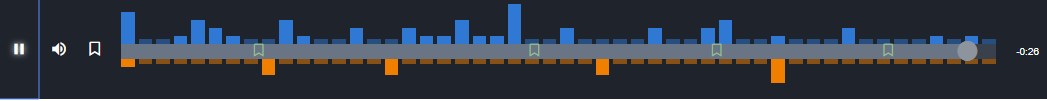
\includegraphics[width=\textwidth,center]{Mediensteuerung.png}
\caption{\label{fig:Mediensteuerung}Darstellung der Mediensteuerung inklusive Visualisierung der Kommentare, Notizen und Lesezeichen}
\end{figure}

\subsection{Suche, Filter und Sortierung bei Kommentaren}
Die elfte Iteration beschäftigte sich mit den gewünschten Such-, Filter- und Sortierungsmöglichkeiten innerhalb der Kommentare und Notizen.

Dafür wurde ein Eingabefeld, zwei Checkboxen und ein Dropdown-Menü in der \textbf{renderer.php} ergänzt. Die Filterung und Sortierung der Daten erfolgte mithilfe eines SQL-Statements, welches der Auflistung \ref{lst:it11:external} zu entnehmen ist. Die einzelnen Funktionen wurden wie folgt umgesetzt:

\begin{itemize}
\item \textbf{Filter}\\
zusätzliche \texttt{WHERE}-Bedingung (Zeile 13):\\
\texttt{comments.comment_type IN (:p_filter_comment, :p_filter_note)}\\
Die Bindevariablen enthalten den jeweiligen Kommentar-Typ, falls dieser angezeigt werden soll und sind sonst leer (vgl. Zeilen 41-42).
\item \textbf{Suche}\\
zusätzliche \texttt{WHERE}-Bedingung (Zeile 14):\\
\texttt{\$DB->sql_like('comments.commenttext', ':p_search_string')}\\
Mithilfe der Funktion \texttt{sql_like} kann überprüft werden, ob der Kommentar den eingegebenen Suchbegriff enthält (vgl. Zeile 43).
\item \textbf{Sortierung}\\
verschiedene \texttt{ORDER BY}-Clauses abhängig von der gewählten Sortierreihenfolge (Zeilen 16-35)\\
Die drei verschiedenen Kriterien werden in entsprechender Reihenfolge angewandt:
\begin{itemize}
\item Annotationszeitpunkte
\item Erstellungszeitpunkte der Original-Kommentare
\item Erstellungszeitpunkte der Antwort-Kommentare
\end{itemize}
\end{itemize}

\begin{lstlisting}[language=php,
             linewidth=\textwidth,
             caption={Ausschnitt der \textbf{external.php} in der 11. Iteration},
             label={lst:it11:external}]
$sql='SELECT comments.id, comments.comment_type, comments.commenttext,'.
    ' comments.timeannotated, comments.timecreated,'.
    ' user.username, comments.comment_id'.
    ' FROM mdl_hyperaudio_comments comments'.
    ' INNER JOIN mdl_user user ON comments.userid = user.id'.
    ' LEFT JOIN mdl_hyperaudio_comments original_comment'.
    ' ON original_comment.id = comments.comment_id'.
    ' WHERE comments.hyperaudio_id = :p_hyperaudio_id'.
    ' AND (comments.comment_type = :p_comment_type_c'.
    ' OR (comments.comment_type = :p_comment_type_note'.
    ' AND comments.userid = :p_userid))'.
    ' AND comments.comment_type'.
    ' IN (:p_filter_comment, :p_filter_note)'.
    ' AND ' . $DB->sql_like('comments.commenttext', ':p_search_string');

switch ($order){
    case timecreated_asc:
        $sql.= 
            'ORDER BY'.
            ' IFNULL(original_comment.timecreated, comments.timecreated) asc,'.
            ' comments.timecreated asc';
        break;
    case timecreated_desc:
        $sql.= 
            'ORDER BY'.
            ' IFNULL(original_comment.timecreated, comments.timecreated) desc,'.
            ' comments.timecreated asc';
        break;
    case timeannotated:
        $sql.=
            'ORDER BY comments.timeannotated asc,'.
            ' IFNULL(original_comment.timecreated, comments.timecreated) asc,'.
            ' comments.timecreated asc';
        break;
}
        
$comments = $DB->get_records_sql($sql, array('p_hyperaudio_id' => $hyperaudio_id,
    'p_comment_type_c' => CommentType::Comment,
    'p_comment_type_note' => CommentType::Note,
    'p_userid' => $USER->id,
    'p_filter_comment' => $filter_comments ? CommentType::Comment : null,
    'p_filter_note' => $filter_notes ? CommentType::Note : null,
    'p_search_string' => '%' . $DB->sql_like_escape($search_string) . '%'));
\end{lstlisting}

Die Umsetzung der Such-, Filter- und Sortierfunktion (siehe Abbildung \ref{fig:Filter}) rundeten die Implementierung der Wiedergabe von Hyperaudio-Dokumenten mit Kommunikations- und Interaktionsmöglichkeiten ab.

\begin{figure}[h!]
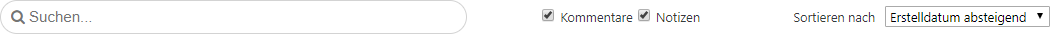
\includegraphics[width=\textwidth,center]{Filter.png}
\caption{\label{fig:Filter}Darstellung der Such-, Filter- und Sortierfunktion}
\end{figure}


%%%%%%%%%%
\subsection{Unterstützung mobiler Endgeräte}
In der letzten Iteration wurden Anpassungen vorgenommen, um die Nutzung des Hyperaudio"=Plugins auch auf mobilen Endgeräte zu ermöglichen. Dafür wurden wie bereits in Abschnitt \ref{sub:mobile} beschrieben Breakpoints eingeführt, um die Anordnung der Elemente für mobile Endgeräte zu optimieren.

Bei geringer Bildschirmbreite werden durch den ersten Breakpoint die Bereiche wie in Abbildung \ref{fig:BereicheDesktopMobile} sichtbar neu angeordnet, sodass statt einem zweispaltigen ein einspaltiges Layout verwendet wird. Das hat zur Folge, dass die Galerie nun unterhalb der Kommentare und Notizen angezeigt wird.

\begin{figure}[h!]
\begin{subfigure}[c]{0.5\textwidth}
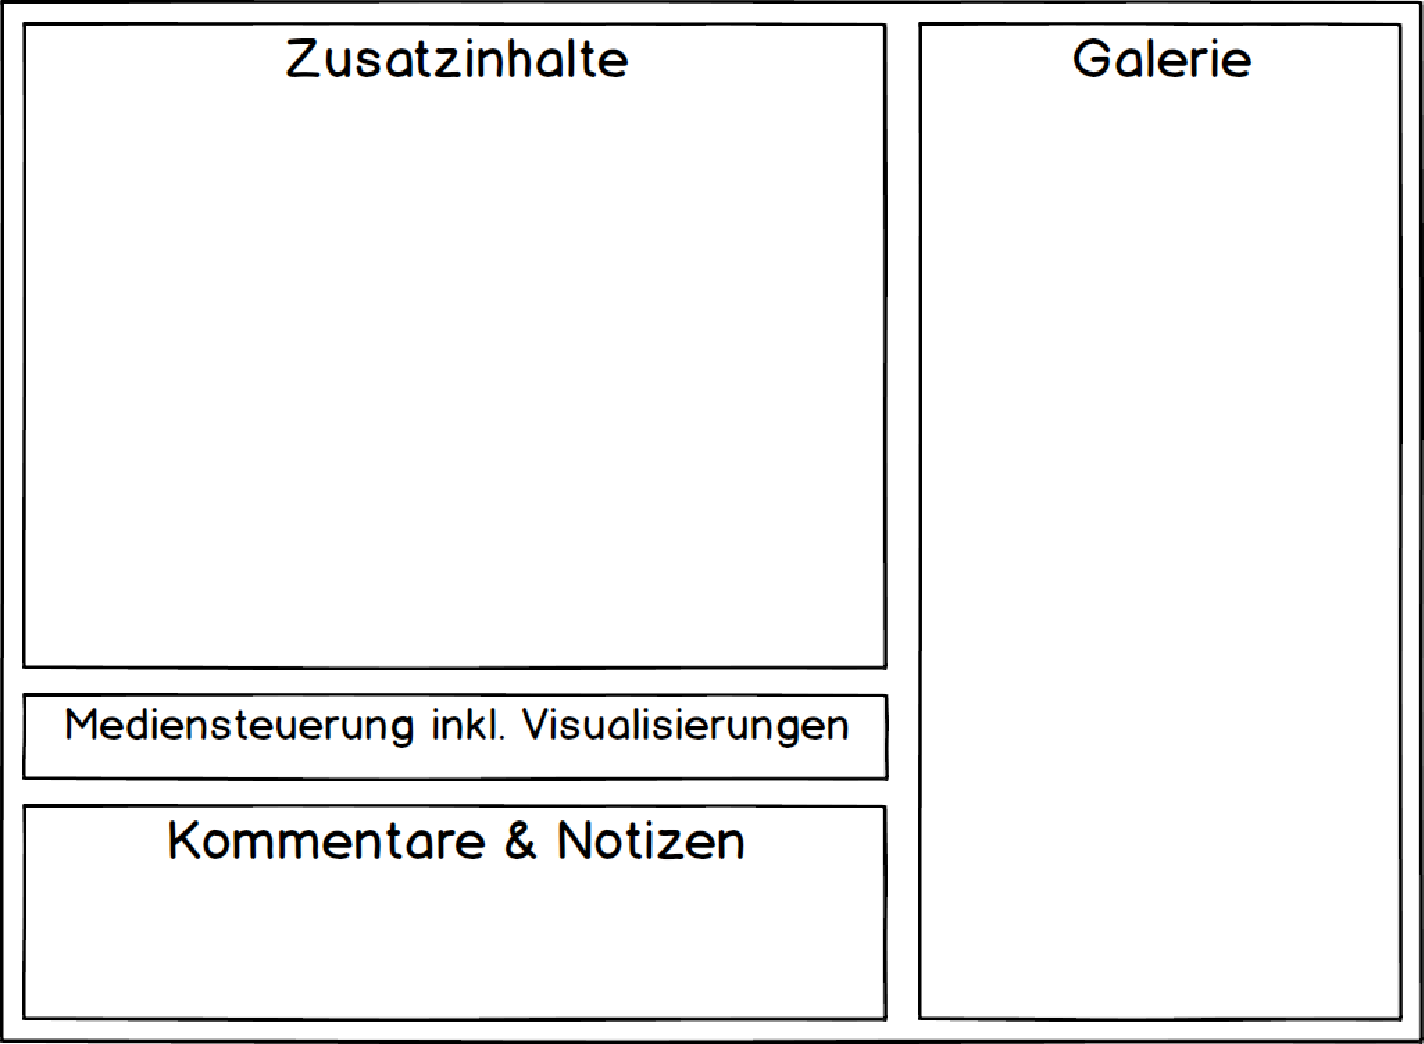
\includegraphics[width=0.95\textwidth,center]{BereicheDesktop.pdf}
\label{fig:BereicheDesktop}
\subcaption{Desktop}
\end{subfigure}%
\begin{subfigure}[c]{0.5\textwidth}
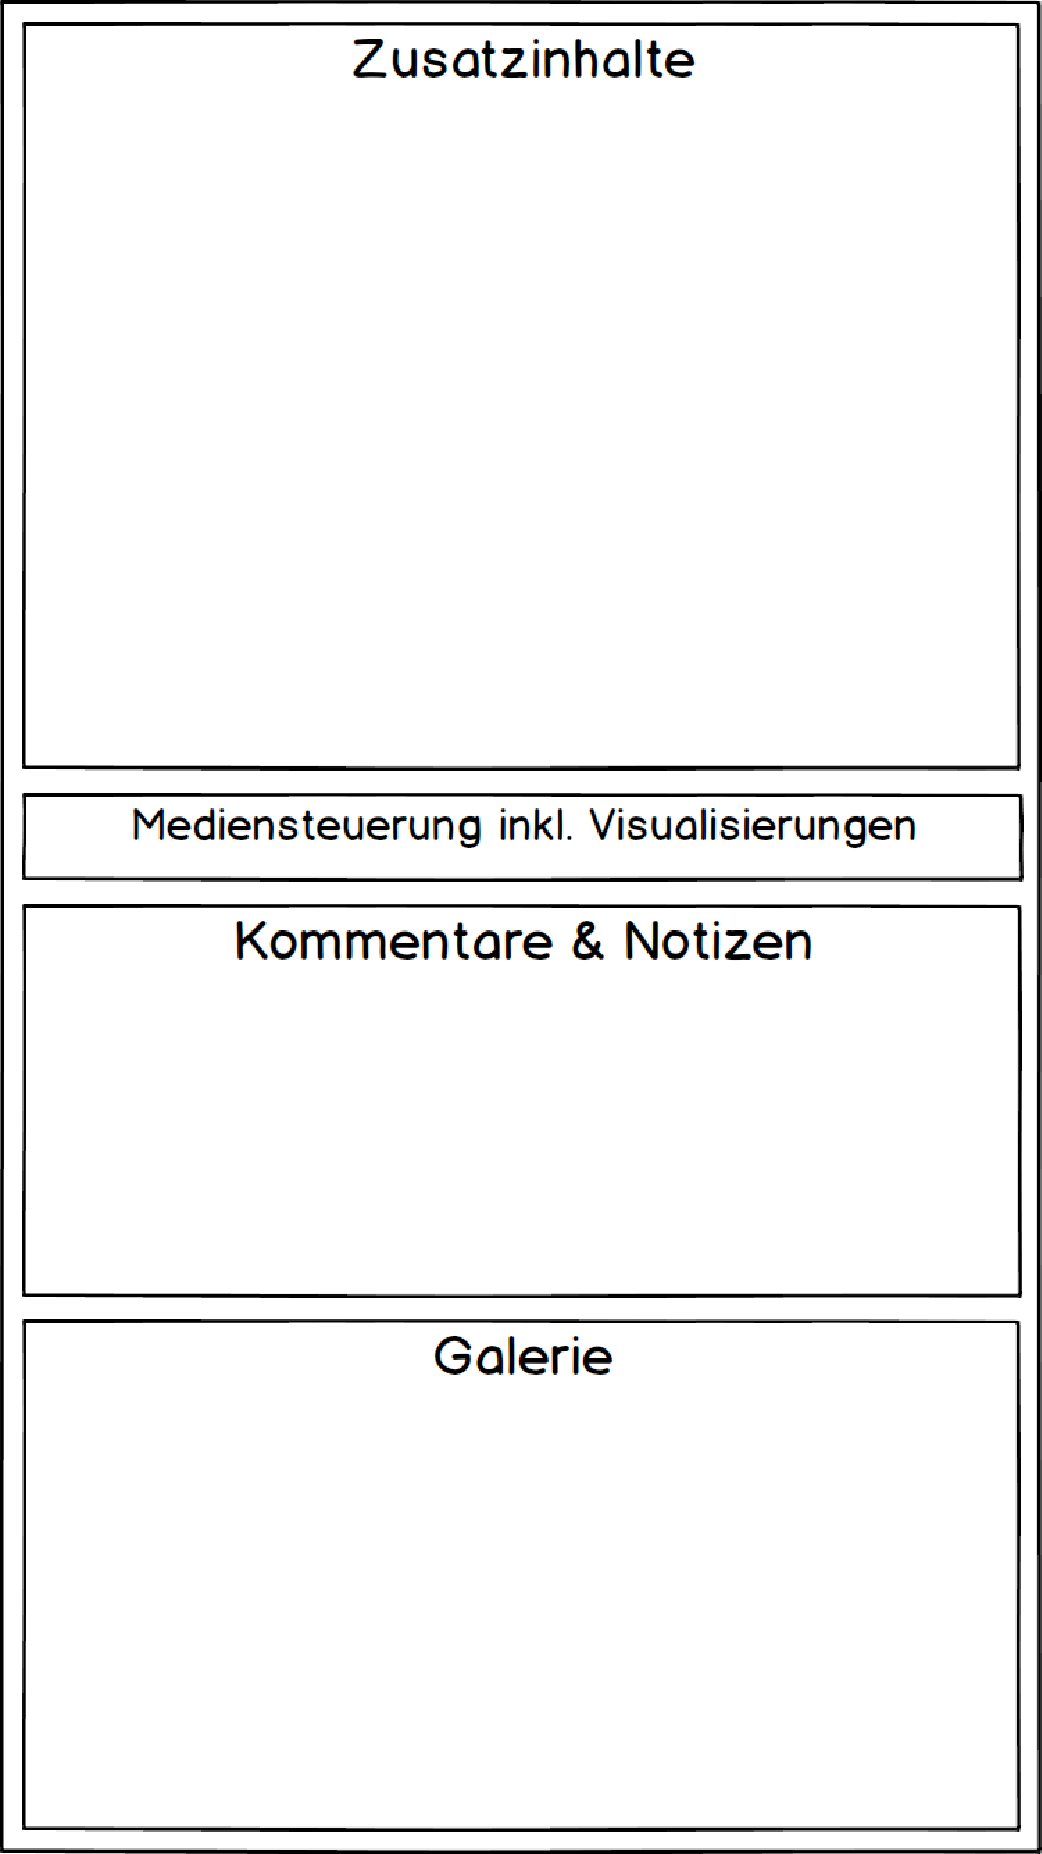
\includegraphics[width=0.6\textwidth,center]{BereicheMobile.pdf}
\label{fig:BereicheMobile}
\subcaption{mobile Endgeräte}
\end{subfigure}
\caption{Darstellung der Bereiche}
\label{fig:BereicheDesktopMobile}
\end{figure}

Ein weiterer Breakpoint wird bei der Such-, Filter- und Sortierfunktion angewandt. Für mobile Endgeräte werden diese Funktionen untereinander statt nebeneinander angeordnet (siehe Abbildung \ref{fig:FilterDesktopMobile}).

\begin{figure}[h!]
\begin{subfigure}[c]{0.5\textwidth}

\includegraphics[width=0.95\textwidth,center]{FilterDesktop.pdf}
\label{fig:FilterDesktop}
\subcaption{Desktop}
\end{subfigure}%
\begin{subfigure}[c]{0.5\textwidth}
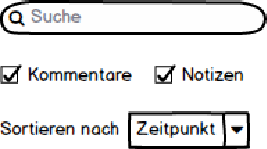
\includegraphics[width=0.6\textwidth,center]{FilterMobile.pdf}
\label{fig:FilterMobile}
\subcaption{mobile Endgeräte}
\end{subfigure}
\caption{Darstellung der Such-, Filter- und Sortierfunktion}
\label{fig:FilterDesktopMobile}
\end{figure}

Um auch innerhalb der Galerie auf die Gegebenheiten von Endgeräten mit geringer Bildschirmbreite Rücksicht zu nehmen, wurde ein weiterer Breakpoint eingeführt. Dieser sorgt dafür, dass die Metainformationen der Zusatzinhalte unterhalb statt neben des Thumbnails dargestellt werden. Hieraus resultiert die in Abbildung \ref{fig:GalerieDesktopMobile} dargestellte Ansicht.

\begin{figure}[h!]
\begin{subfigure}[c]{0.5\textwidth}
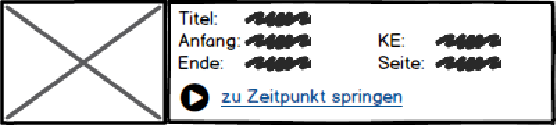
\includegraphics[width=0.95\textwidth,center]{GalerieDesktop.pdf}
\label{fig:GalerieDesktop}
\subcaption{Desktop}
\end{subfigure}%
\begin{subfigure}[c]{0.5\textwidth}
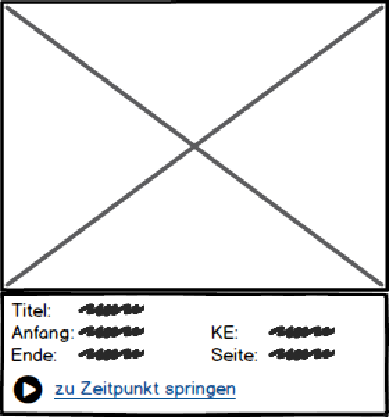
\includegraphics[width=0.6\textwidth,center]{GalerieMobile.pdf}
\label{fig:GalerieMobile}
\subcaption{mobile Endgeräte}
\end{subfigure}
\caption{Darstellung der Galerie}
\label{fig:GalerieDesktopMobile}
\end{figure}

\FloatBarrier

Umgesetzt wurden diese Breakpoints anhand von CSS-Regeln innerhalb der \textbf{styles.css} (siehe Auflistung \ref{lst:it12:styles}). Die verschiedenen Darstellungen werden mittels Medienabfragen gesteuert. Dabei wird die Breite des Anzeigebereichs abgefragt und falls die angegebene Grenze überschritten wird, werden die innerhalb des \texttt{@media}-Blocks definierten Regeln angewandt. Diese  erzeugen mittels Grid Layout die Desktop-Darstellungsvariante. Andernfalls gelten die \glqq normalen\grqq{} CSS-Regeln, welche die Darstellung auf mobilen Endgeräten definieren.

\begin{lstlisting}[language=css,
             linewidth=\textwidth,
             caption={Ausschnitt der \textbf{styles.css} in der 12. Iteration},
             label={lst:it12:styles}]
@media (min-width: 100em) {
  div#hyperaudio div#hyperaudio {
    display: grid;
    grid-template-columns: 70em 1fr;
  }
  div#hyperaudio div#gallery_container {
    margin-left: 2em;
  }
}
@media (min-width: 40em) {
  div#hyperaudio div.gallery_additional_content {
    display: grid;
    grid-template-columns: 1fr 5fr;
  }
}
@media (min-width: 50em) {
  div#hyperaudio div#comment_tools_container {
    display: grid;
    grid-template-columns: 4fr 2fr 3fr;
  }
  div#hyperaudio input#hyperaudio_search {
  	max-width: 35em;
  	margin-top: 0em;
  }
  div#hyperaudio div#comment_tools_filter,
  div#hyperaudio div#comment_tools_order {
  	display: flex;
    justify-content: flex-end;
    margin-left: 20px;
  }
}
div#hyperaudio div.gallery_additional_content {
    margin-bottom: 15px;
    padding: 5px 10px;
    border-radius: 10px;
}
div#hyperaudio div#comment_tools_container {
    align-items: baseline;
    margin-top: 1rem;
    max-width: 70em;
}
div#hyperaudio input#hyperaudio_search {
    font-family: Arial, FontAwesome;
    font-weight: normal;
    padding: 5px 10px;
    border: 1px solid lightgray;
    border-radius: 20px;
    width: 100%;
    margin-top: 0.3em;
}
div#hyperaudio div#comment_tools_order {
    align-items: baseline;
}
\end{lstlisting}

\begin{figure}[h!]
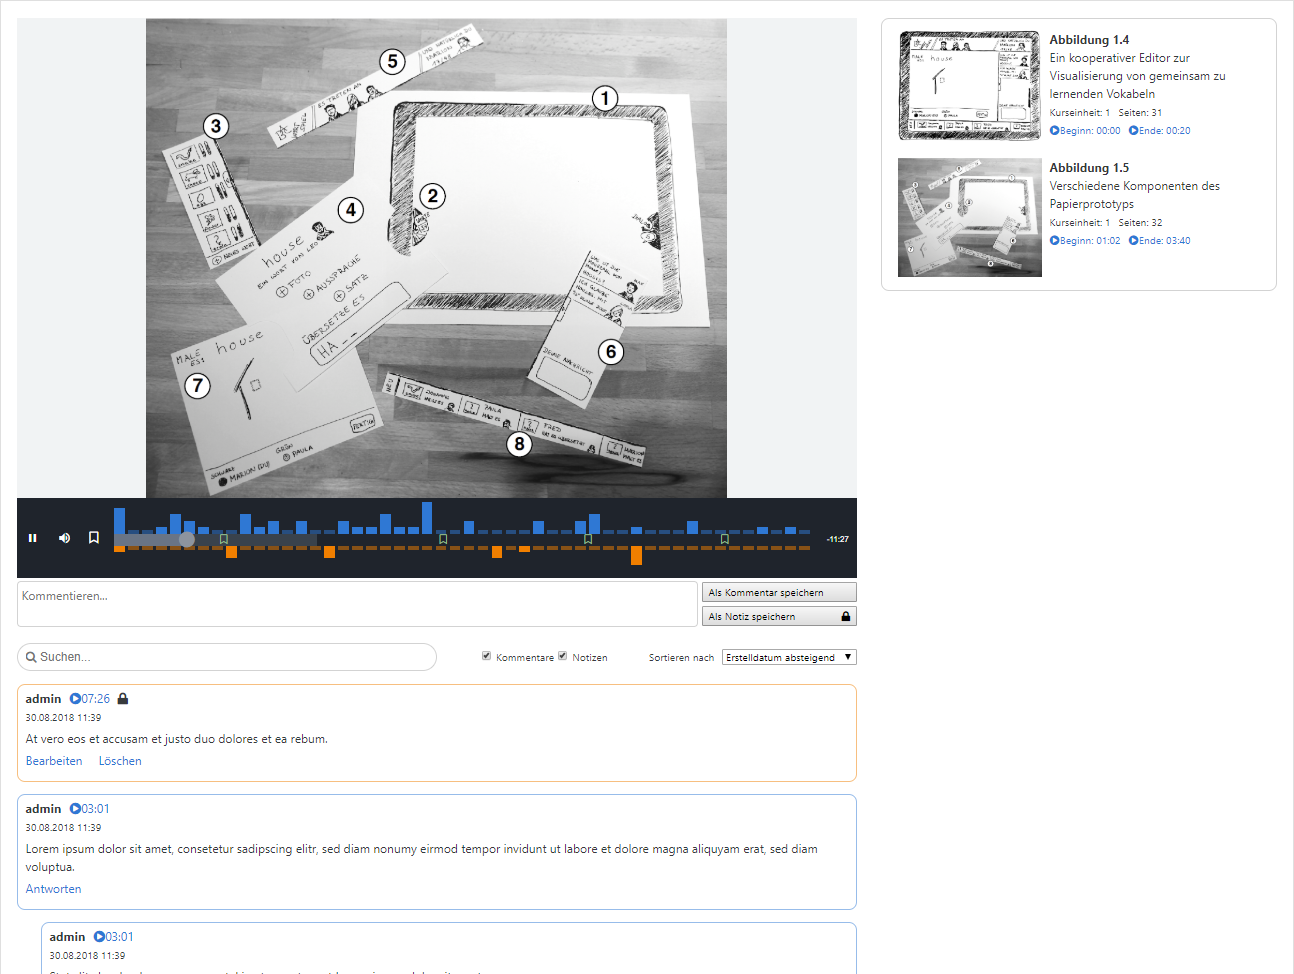
\includegraphics[width=0.85\textwidth,center]{Desktop.png}
\caption{\label{fig:DesktopFinal}Darstellung der finalen Desktop-Version}
\end{figure}

\begin{figure}[h!]
\begin{subfigure}[c]{0.5\textwidth}
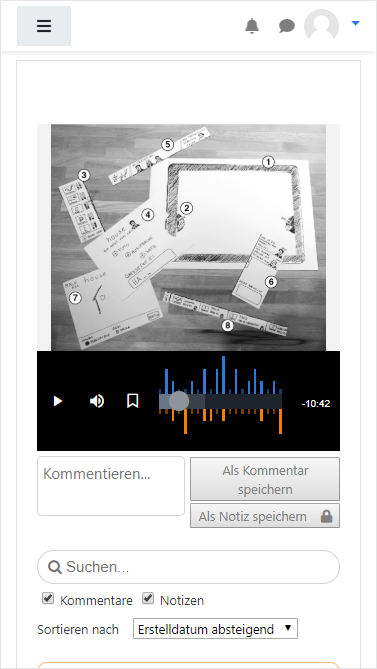
\includegraphics[width=0.9\textwidth,center]{Mobil1.png}
\end{subfigure}%
\begin{subfigure}[c]{0.5\textwidth}
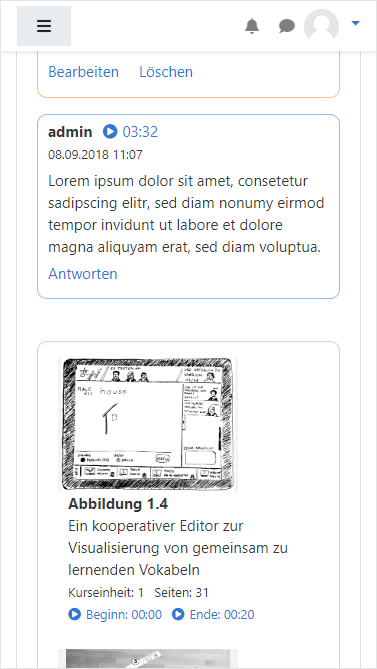
\includegraphics[width=0.9\textwidth,center]{Mobil2.png}
\end{subfigure}
\caption{Darstellung der finalen mobilen Version}
\label{fig:MobilFinal}
\end{figure}

\FloatBarrier

%%%%%%%%%%
\section{Zusammenfassung}
Nachdem zu Beginn der Implementierung die grundlegende Moodle-Struktur erarbeitet wurde, wurden in den darauffolgenden Iterationen das Hyperaudio"=Plugin Schritt für Schritt um die einzelnen Anforderungen erweitert. Somit ist am Ende die in Abbildung \ref{fig:DesktopFinal} sichtbar finale Repräsentation von Kurseinheiten als Hyperaudio"=Dokumente innerhalb eines Moodle-Plugins entstanden. In der letzten Iteration wurde dann noch die Darstellung auf mobilen Endgeräten implementiert.
